\documentclass[12pt]{beamer}\usepackage{graphicx, color}
%% maxwidth is the original width if it is less than linewidth
%% otherwise use linewidth (to make sure the graphics do not exceed the margin)
\makeatletter
\def\maxwidth{ %
  \ifdim\Gin@nat@width>\linewidth
    \linewidth
  \else
    \Gin@nat@width
  \fi
}
\makeatother

\definecolor{fgcolor}{rgb}{0.2, 0.2, 0.2}
\newcommand{\hlnumber}[1]{\textcolor[rgb]{0,0,0}{#1}}%
\newcommand{\hlfunctioncall}[1]{\textcolor[rgb]{0.501960784313725,0,0.329411764705882}{\textbf{#1}}}%
\newcommand{\hlstring}[1]{\textcolor[rgb]{0.6,0.6,1}{#1}}%
\newcommand{\hlkeyword}[1]{\textcolor[rgb]{0,0,0}{\textbf{#1}}}%
\newcommand{\hlargument}[1]{\textcolor[rgb]{0.690196078431373,0.250980392156863,0.0196078431372549}{#1}}%
\newcommand{\hlcomment}[1]{\textcolor[rgb]{0.180392156862745,0.6,0.341176470588235}{#1}}%
\newcommand{\hlroxygencomment}[1]{\textcolor[rgb]{0.43921568627451,0.47843137254902,0.701960784313725}{#1}}%
\newcommand{\hlformalargs}[1]{\textcolor[rgb]{0.690196078431373,0.250980392156863,0.0196078431372549}{#1}}%
\newcommand{\hleqformalargs}[1]{\textcolor[rgb]{0.690196078431373,0.250980392156863,0.0196078431372549}{#1}}%
\newcommand{\hlassignement}[1]{\textcolor[rgb]{0,0,0}{\textbf{#1}}}%
\newcommand{\hlpackage}[1]{\textcolor[rgb]{0.588235294117647,0.709803921568627,0.145098039215686}{#1}}%
\newcommand{\hlslot}[1]{\textit{#1}}%
\newcommand{\hlsymbol}[1]{\textcolor[rgb]{0,0,0}{#1}}%
\newcommand{\hlprompt}[1]{\textcolor[rgb]{0.2,0.2,0.2}{#1}}%

\usepackage{framed}
\makeatletter
\newenvironment{kframe}{%
 \def\at@end@of@kframe{}%
 \ifinner\ifhmode%
  \def\at@end@of@kframe{\end{minipage}}%
  \begin{minipage}{\columnwidth}%
 \fi\fi%
 \def\FrameCommand##1{\hskip\@totalleftmargin \hskip-\fboxsep
 \colorbox{shadecolor}{##1}\hskip-\fboxsep
     % There is no \\@totalrightmargin, so:
     \hskip-\linewidth \hskip-\@totalleftmargin \hskip\columnwidth}%
 \MakeFramed {\advance\hsize-\width
   \@totalleftmargin\z@ \linewidth\hsize
   \@setminipage}}%
 {\par\unskip\endMakeFramed%
 \at@end@of@kframe}
\makeatother

\definecolor{shadecolor}{rgb}{.97, .97, .97}
\definecolor{messagecolor}{rgb}{0, 0, 0}
\definecolor{warningcolor}{rgb}{1, 0, 1}
\definecolor{errorcolor}{rgb}{1, 0, 0}
\newenvironment{knitrout}{}{} % an empty environment to be redefined in TeX

\usepackage{alltt}

\usetheme{Madrid}
%\usecolortheme{seahorse}
\usepackage[spanish]{babel}
\usepackage[latin1]{inputenc}


\title{Experiencia Uso de {\fontfamily{phv}\selectfont R} para An�lsis Espacial}
\author{Francisco Zambrano Bigiarini}

\date{\today}
\IfFileExists{upquote.sty}{\usepackage{upquote}}{}

\begin{document}

\begin{frame}
\titlepage
\end{frame}

\begin{frame}{Introducci�n}
\begin{itemize}[<+->]
\item La informaci�n espacial se encuentra en todas partes.
\item Por mas de 10 a�os hubo una creciente contribuci�n de paquetes para manejar y analizar informaci�n espacial.
\item 2005: Un grupo de desarrolladores de R crearon el paquete 'sp' para extender R con metodos y clases para an�lisis espacial.
\item Applied Spatial Data Analysis with R: Roger Bivand, Edzer Pebesma and Virgilio G�mez-Rubio.
\end{itemize}
\pause
\begin{center}
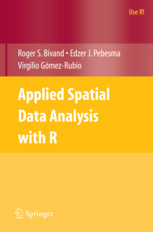
\includegraphics[width=2.5cm]{imagenes/libro_spatial.jpg}
\end{center}
\end{frame}

\begin{frame}{Introducci�n}
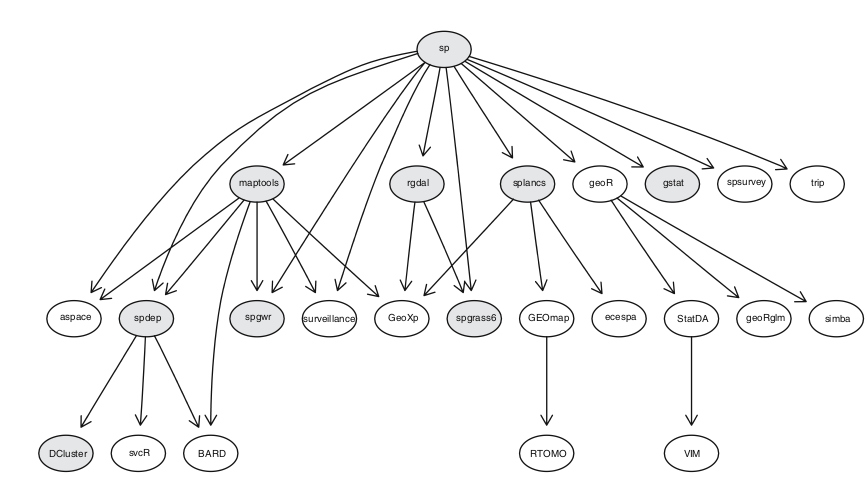
\includegraphics[width=\textwidth]{imagenes/red_sp.png}
\end{frame}


\begin{frame}[fragile]{Manejo de Informaci�n Espacial con \textbf{sp}}
Data frame con informaci�n espacial: coordenadas geogr�ficas (x, y) y variables con distintos parametros (cadmio, cobre, plomo, etc)
\begin{knitrout}\scriptsize
\definecolor{shadecolor}{rgb}{0.969, 0.969, 0.969}\color{fgcolor}\begin{kframe}
\begin{alltt}
> \hlfunctioncall{require}(sp)
> \hlfunctioncall{data}(meuse)
> \hlfunctioncall{str}(meuse)
\end{alltt}
\begin{verbatim}
## 'data.frame':	155 obs. of  14 variables:
##  $ x      : num  181072 181025 181165 181298 181307 ...
##  $ y      : num  333611 333558 333537 333484 333330 ...
##  $ cadmium: num  11.7 8.6 6.5 2.6 2.8 3 3.2 2.8 2.4 1.6 ...
##  $ copper : num  85 81 68 81 48 61 31 29 37 24 ...
##  $ lead   : num  299 277 199 116 117 137 132 150 133 80 ...
##  $ zinc   : num  1022 1141 640 257 269 ...
##  $ elev   : num  7.91 6.98 7.8 7.66 7.48 ...
##  $ dist   : num  0.00136 0.01222 0.10303 0.19009 0.27709 ...
##  $ om     : num  13.6 14 13 8 8.7 7.8 9.2 9.5 10.6 6.3 ...
##  $ ffreq  : Factor w/ 3 levels "1","2","3": 1 1 1 1 1 1 1 1 1 1 ...
##  $ soil   : Factor w/ 3 levels "1","2","3": 1 1 1 2 2 2 2 1 1 2 ...
##  $ lime   : Factor w/ 2 levels "0","1": 2 2 2 1 1 1 1 1 1 1 ...
##  $ landuse: Factor w/ 15 levels "Aa","Ab","Ag",..: 4 4 4 11 4 11 4 2 2 15 ...
##  $ dist.m : num  50 30 150 270 380 470 240 120 240 420 ...
\end{verbatim}
\end{kframe}
\end{knitrout}

\end{frame}

\begin{frame}[fragile]{Manejo de Informaci�n Espacial con \textbf{sp}}
El data frame puede transformarce a informaci�n espacial con la funci�n \textbf{coordinates}.
El data frame pasa a ser ahora un 'SpatialPointsDataFrame' con una estructura diferente.
\begin{knitrout}\tiny
\definecolor{shadecolor}{rgb}{0.969, 0.969, 0.969}\color{fgcolor}\begin{kframe}
\begin{alltt}
> \hlfunctioncall{coordinates}(meuse) <- ~x + y
> \hlfunctioncall{str}(meuse)
\end{alltt}
\begin{verbatim}
## Formal class 'SpatialPointsDataFrame' [package "sp"] with 5 slots
##   ..@ data       :'data.frame':	155 obs. of  12 variables:
##   .. ..$ cadmium: num [1:155] 11.7 8.6 6.5 2.6 2.8 3 3.2 2.8 2.4 1.6 ...
##   .. ..$ copper : num [1:155] 85 81 68 81 48 61 31 29 37 24 ...
##   .. ..$ lead   : num [1:155] 299 277 199 116 117 137 132 150 133 80 ...
##   .. ..$ zinc   : num [1:155] 1022 1141 640 257 269 ...
##   .. ..$ elev   : num [1:155] 7.91 6.98 7.8 7.66 7.48 ...
##   .. ..$ dist   : num [1:155] 0.00136 0.01222 0.10303 0.19009 0.27709 ...
##   .. ..$ om     : num [1:155] 13.6 14 13 8 8.7 7.8 9.2 9.5 10.6 6.3 ...
##   .. ..$ ffreq  : Factor w/ 3 levels "1","2","3": 1 1 1 1 1 1 1 1 1 1 ...
##   .. ..$ soil   : Factor w/ 3 levels "1","2","3": 1 1 1 2 2 2 2 1 1 2 ...
##   .. ..$ lime   : Factor w/ 2 levels "0","1": 2 2 2 1 1 1 1 1 1 1 ...
##   .. ..$ landuse: Factor w/ 15 levels "Aa","Ab","Ag",..: 4 4 4 11 4 11 4 2 2 15 ...
##   .. ..$ dist.m : num [1:155] 50 30 150 270 380 470 240 120 240 420 ...
##   ..@ coords.nrs : int [1:2] 1 2
##   ..@ coords     : num [1:155, 1:2] 181072 181025 181165 181298 181307 ...
##   .. ..- attr(*, "dimnames")=List of 2
##   .. .. ..$ : NULL
##   .. .. ..$ : chr [1:2] "x" "y"
##   ..@ bbox       : num [1:2, 1:2] 178605 329714 181390 333611
##   .. ..- attr(*, "dimnames")=List of 2
##   .. .. ..$ : chr [1:2] "x" "y"
##   .. .. ..$ : chr [1:2] "min" "max"
##   ..@ proj4string:Formal class 'CRS' [package "sp"] with 1 slots
##   .. .. ..@ projargs: chr NA
\end{verbatim}
\end{kframe}
\end{knitrout}

\end{frame}

\begin{frame}[fragile]{Manejo de Informaci�n Espacial con \textbf{sp}}
Utilizando \textbf{'CRS'} para definir la projecci�n de la informaci�n espacial y \textbf{'proj4string'} para asignar 
la projecci�n a \textbf{'meuse'}
\begin{knitrout}\scriptsize
\definecolor{shadecolor}{rgb}{0.969, 0.969, 0.969}\color{fgcolor}\begin{kframe}
\begin{alltt}
> crs = \hlfunctioncall{CRS}(\hlstring{"+init=epsg:28992 +proj=sterea +lat_0=52.15616055555555\textbackslash{}n+lon_0=5.38763888888889 +k=0.9999079\textbackslash{}n+x_0=155000 +y_0=463000 +ellps=bessel\textbackslash{}n+towgs84=565.417,50.3319,465.552,-0.398957,0.343988,-1.8774,4.0725\textbackslash{}n+units=m +no_defs"})
> \hlfunctioncall{proj4string}(meuse) <- crs
> \hlfunctioncall{library}(lattice)
> \hlfunctioncall{trellis.par.set}(\hlfunctioncall{sp.theme}())  \hlcomment{# sets \hlfunctioncall{bpy.colors}() ramp}
> l2 = \hlfunctioncall{list}(\hlstring{"SpatialPolygonsRescale"}, \hlfunctioncall{layout.north.arrow}(), offset = \hlfunctioncall{c}(181300, 
+     329800), scale = 400)
> l3 = \hlfunctioncall{list}(\hlstring{"SpatialPolygonsRescale"}, \hlfunctioncall{layout.scale.bar}(), offset = \hlfunctioncall{c}(180500, 329800), 
+     scale = 500, fill = \hlfunctioncall{c}(\hlstring{"transparent"}, \hlstring{"black"}))
> l4 = \hlfunctioncall{list}(\hlstring{"sp.text"}, \hlfunctioncall{c}(180500, 329900), \hlstring{"0"})
> l5 = \hlfunctioncall{list}(\hlstring{"sp.text"}, \hlfunctioncall{c}(181000, 329900), \hlstring{"500 m"})
\end{alltt}
\end{kframe}
\end{knitrout}

\end{frame}

\begin{frame}[fragile]{Manejo de Informaci�n Espacial con \textbf{sp}}
Un simple gr�fico de la informaci�n espacial para las concentraciones de \textbf{'zinc'} y \textbf{'plomo'} con la funci�n \textbf{'spplot'}
\begin{knitrout}\tiny
\definecolor{shadecolor}{rgb}{0.969, 0.969, 0.969}\color{fgcolor}\begin{kframe}
\begin{alltt}
\hlfunctioncall{spplot}(meuse, \hlfunctioncall{c}(\hlstring{"zinc"}, \hlstring{"lead"}), sp.layout = \hlfunctioncall{list}(l2, l3, l4, l5, which = 2), 
    key.space = \hlfunctioncall{list}(x = 0.1, y = 0.95, corner = \hlfunctioncall{c}(0, 1)))
\end{alltt}
\end{kframe}

{\centering 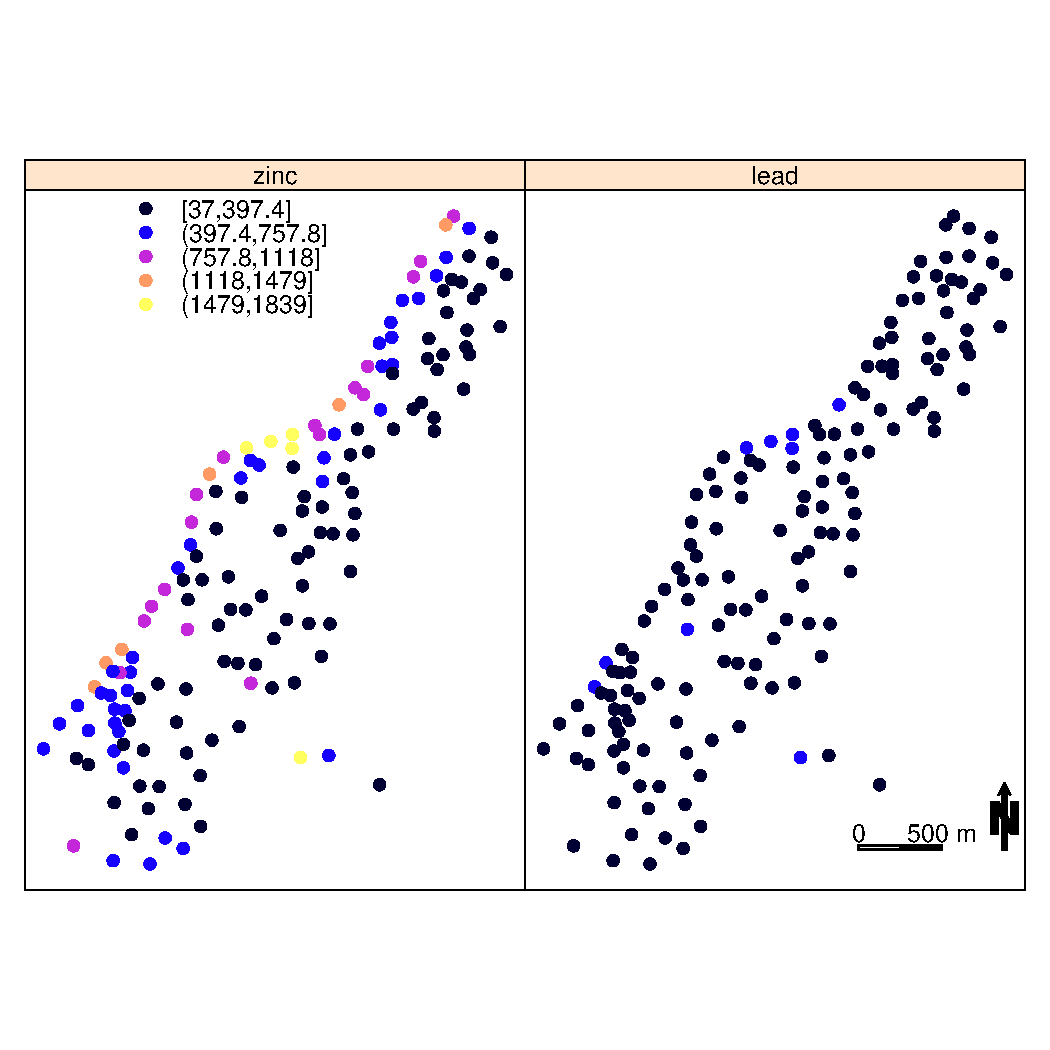
\includegraphics[width=0.65\linewidth]{figure/unnamed-chunk-4} 

}



\end{knitrout}

\end{frame}


\begin{frame}[fragile]{Algo con el paquete \textbf{'raster'}}
Cargando seis im�genes en la variable 'x', como objeto \textbf{'RasterStack'}
\begin{knitrout}\tiny
\definecolor{shadecolor}{rgb}{0.969, 0.969, 0.969}\color{fgcolor}\begin{kframe}
\begin{alltt}
> \hlfunctioncall{library}(raster)
> x <- \hlfunctioncall{stack}(\hlfunctioncall{paste}(\hlstring{"raster/"}, \hlfunctioncall{list.files}(\hlstring{"raster"}), sep = \hlstring{""})[1:6])
> \hlfunctioncall{summary}(x)
\end{alltt}
\begin{verbatim}
##         MOD13A1.A2000049.chl.3585 MOD13A1.A2000065.chl.3585
## Min.                         2454                      2876
## 1st Qu.                      4760                      5104
## Median                       5716                      5960
## 3rd Qu.                      7404                      7307
## Max.                         9099                      9102
## NA's                         1851                      1851
##         MOD13A1.A2000081.chl.3585 MOD13A1.A2000097.chl.3585
## Min.                         3015                      2977
## 1st Qu.                      5142                      5114
## Median                       5985                      5982
## 3rd Qu.                      7287                      7290
## Max.                         9066                      9213
## NA's                         1851                      1851
##         MOD13A1.A2000113.chl.3585 MOD13A1.A2000129.chl.3585
## Min.                         3125                      3232
## 1st Qu.                      5127                      5255
## Median                       5968                      5966
## 3rd Qu.                      7221                      6895
## Max.                         9143                      9296
## NA's                         1851                      1851
\end{verbatim}
\end{kframe}
\end{knitrout}

\end{frame}

\begin{frame}[fragile]{Algo con el paquete \textbf{'raster'}}
Utilizando el m�todo plot para un objeto de clase \textbf{'RasterStack'}
\begin{knitrout}
\definecolor{shadecolor}{rgb}{0.969, 0.969, 0.969}\color{fgcolor}\begin{kframe}
\begin{alltt}
\hlfunctioncall{plot}(x)
\end{alltt}
\end{kframe}
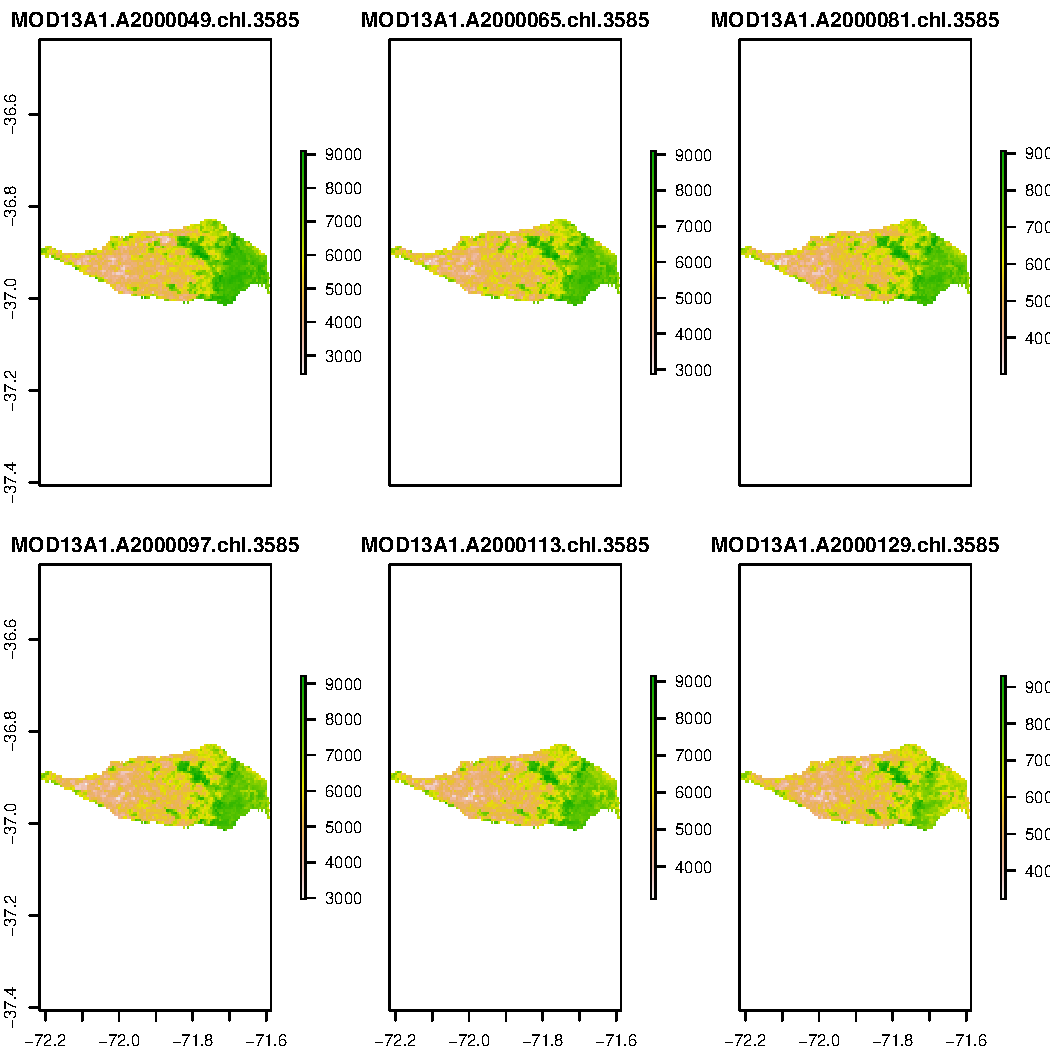
\includegraphics[width=\linewidth,height=0.7\textheight]{figure/unnamed-chunk-5} 

\end{knitrout}

\end{frame}

\begin{frame}[fragile]{Algo con el paquete \textbf{'raster'}}
Funci�n 'fivenum' aplicada a traves de la funci�n 'calc' del paquete raster
\begin{knitrout}\tiny
\definecolor{shadecolor}{rgb}{0.969, 0.969, 0.969}\color{fgcolor}\begin{kframe}
\begin{alltt}
result <- \hlfunctioncall{calc}(x, \hlfunctioncall{function}(x) \hlfunctioncall{fivenum}(x))
\hlfunctioncall{plot}(result)
\end{alltt}
\end{kframe}
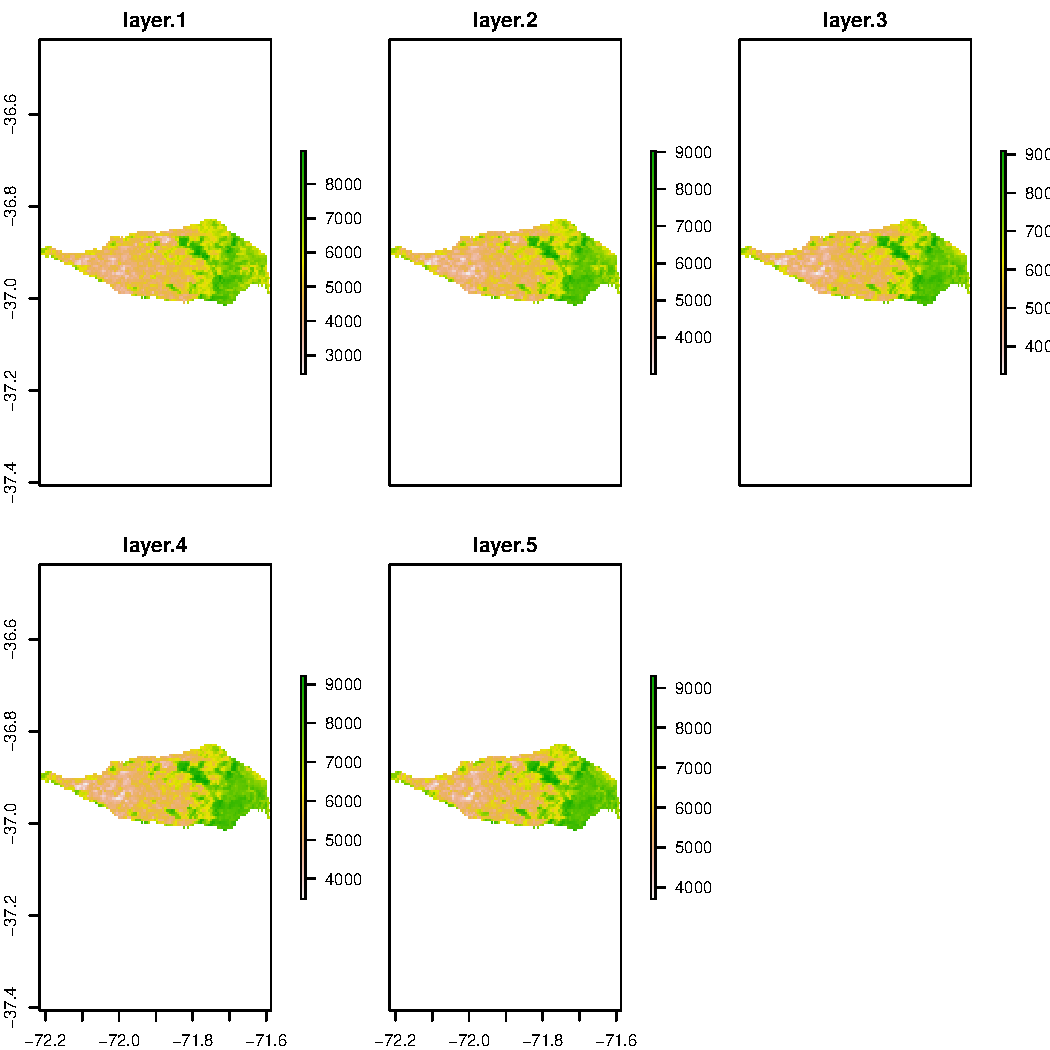
\includegraphics[width=\linewidth,height=0.7\textheight]{figure/unnamed-chunk-6} 

\end{knitrout}

\end{frame}

\begin{frame}{De que me ha servido el uso de informaci�n espacial y raster en 'R'}
\begin{itemize}[<+->]
\item Dejar de utilizar software de pago como: ArcGis, Envi, Erdas, etc.
\item Procesar im�genes MODIS de todo Chile entre 2000-2012.
\item La superficie total de chile corresponde a 12 MM de pixeles para una resoluci�n de 250m
\item Se utilizan 300 imagenes aprox, frecuencia de 16 dias
\item Se realiza un suavizado para cada pixel para la serie temporal ('lowess' o 'loess').
\item Se calculan los resumen estadistico (fivenum,boxplot.stats,etc) para la serie completa.
\item Se calcula diferentes indices vegetacionales y de sequ�a
\item ...
\end{itemize}
\end{frame}

\begin{frame}{Datos de Utilidad}
\begin{enumerate}
\item Pebesma, E.J., 2004. Multivariable geostatistics in S: the gstat package. Computers & Geosciences, 30: 683-691.
\item Hengl, Tomislav. 2009. A practical guide to geostatistical mapping. \url{spatial-analyst.net}
\item Grupo de correo [R-SIG-GEO]
\item Algunos paquetes interesantes: maptools, rgdal, rasterVIS, plotKML, gstat, MODIS.
\end{enumerate}
\end{frame}

\end{document}
